\Huge\textbf{Capitolo 3: \\ Struttura della membrana}

\section{Lipidi}
    \small
    I lipidi sono una classe di biomolecole che sono caratterizzate da una porzione idrofoba. 
    
    \subsection{Acidi grassi}
        Gli acidi grassi sono una categoria di lipidi caratterizzati da una coda idrocarburica più o meno lunga associata a una testa idrofilica. In se stesso racchiude la caratteristica anfipatica.
        Qualora compaiano doppi legami tra i carboni della coda, si dice che l'acido grasso è \textit{insaturo}, si dice \textit{saturo} altrimenti. La presenza di code insature favoriscono il comportamento liquido della membrana, al contrario, la presenza di catene sature favorisce la rigidità.
        
    \subsection{Fosfolipidi}
        I fosfolipidi sono una classe di lipidi composti da catene di acido grasso e una testa di glicerolo: la testa è fortemente idrofila mentre la coda fortemente idrofobica.
        Questa struttura conferisce la caratteristica \textit{anfipatica} alla molecola e si associa spontaneamente nella formazione di membrana con core idrofobico e esternamente carattere idrofilo.\\
        La \textit{fosfatidilcolina} è il fosfolipide più abbondante nelle membrane, è composto di colina, fosfato, glicerolo e due code idrofobiche.
        \subsubsection{Fosfogliceridi}
            Sono una categoria di fosfolipidi che si differenziano tra loro in base alla composizione della testa polare, alla quale si aggiunge il di-acil-glicerolo presenti in maggioranza tra i lipidi di membrana. Tra queste possiamo ricordare \textit{fosfatidil serina}, \textit{fosfatidil etanolammina}, \textit{fosfatidil inositolo} e \textit{fosfatidil colina}.\\
            
            \textbf{Plasmalogeni}\\
                Sono una sottoclasse di fosfolipidi caratterizzata da un gruppo vinil-etere in posizione 1 del glicerolo. Le catene idrocarburiche sono legate una tramite un legame etere e una tramite legame estere.\\
            
            \textbf{Sfingolipidi}\\
                Sono una categoria di fosfolipidi, che al posto del glicerolo contengono sfingosina e una testa polare, alla quale è legata una catena acida, un gruppo amminico e due gruppi ossidrili. Sono anche esse molecole anfipatiche. Hanno la possibilità di essere glicosilati.
        
    \subsection{Trigliceridi}
        Sono una categoria di lipidi scarsamente anfipatica, proprio per questo motivo non fanno parte della membrana cellulare. Consiste di un glicerolo associato a tre acidi grassi ed è fortemente idrofoba. La loro funzione è la conservazione dell'energia sottoforma di accumulo.\\
        I depositi di grassi all'interno della cellula vengono generati a livello di membrana, a livello della quale si forma un'invaginazione monolayer (foglietto citosolico) contenente trigliceridi o colesterolo. Successivamente viene estrusa a formare un monostrato lipidico, quindi una gocciolina di grasso.\\
        Gli acidi grassi dei trigliceridi possono essere lineari o "piegati" in base alla presenza o assenza dei doppi legami (insaturi). Il livello di insaturazione inferisce determinate caratteristiche chimiche-fisiche (ad esempio la temperatura di fusione).
        
    \subsection{Steroli}
        Sono una categoria di lipidi presenti negli animali (gli analoghi vegetale sono ergosterolo e stigmasterolo).
        Sono composti da quattro anelli idrocarburici e una coda idrocarburica non polare.\\
        Anche questa categoria presenta caratteristiche anfipatiche dovute alla presenza di un gruppo ossidrile dal lato opposto della catena.\\
        Sono di dimensioni inferiori rispetto ai fosfolipidi, sono presenti nel doppio strato lipidico della membrana: il gruppo OH dello sterolo interagisce con la testa polare dei fosfolipidi e costituiscono una componente più interna.\\
        La funzione di queste molecole all'interno della membrana è legata alla fluidità del mosaico: una maggior concentrazione aumenta la rigidità (nel caso si introducano artificialmente si assiste al comportamento inverso). 
        La presenza del colesterolo previene la diffusione (aumenta viscosità) due-dimensionale dei componenti attraverso la membrana e concorre alla formazione di microdomini con caratteristiche fisiche diverse sulla membrana.
        
    \subsection{Glicolipidi}
        I glicolipidi sono una categoria di lipidi che contengono uno zucchero come residuo legato alla testa polare. Sono presenti solo nello strato esterno della membrana. L'aggiunta dello zucchero avviene a livello del Golgi. \\
        La loro funzione comprende l'interazione tra la cellula e l'ambiente, sono punti di ingresso per tossine e sono utili per cariche elettriche e pH.
    
\section{Doppio strato lipidico}
    La membrana plasmatica consiste di un doppio strato lipidico, formato prevalentemente da fosfogliceridi, steroli, glicolipidi e sfingolipidi, tuttavia sono presenti anche molte proteine. Tutte le molecole che formano la membrana sono anfipatiche. 
    Tra i lipidi citati, i primi sono i più abbondanti. Ha la funzione di filtro, ricevere informazioni, media selettivamente entrata e uscita di molecole e delimita la cellula stessa.\\
    La struttura planare di doppio strato lipidico è energicamente sfavorita, se la si pone in soluzione infatti tenderà a richiudersi spontaneamente su se stessa formando un liposoma (detti micelle qualora non contengano all'interno soluzione acquosa) minimizzando l'interazione con il solvente.\\
    Il liposoma viene utilizzato per studiare il contenuto della membrana. Si possono formare a partire da una membrana biologica (includendo componente proteica), scomporla con componenti organici che portano alla precipitazione delle proteine e riportando in soluzione acquosa i lipidi che tenderanno a formare un liposoma.
    In alternativa ci sono strumenti per formare un bilayer a cavallo di un foro in soluzione acquosa, simulare quindi un compartimento intracellulare e extracellulare.\\
    Elementi proteici associati alla membrana sono responsabili dell'interazione con il citoscheletro e quindi dettano la morfologia.\\
    
    I vari tipi di lipidi sono presenti in percentuali differenti in membrane di cellule differenti differenti. 
    Membrane diverse hanno composizioni diverse, quindi proprietà biofisiche diverse. \\
    Per esempio la sfingomielina è presente al 13\% nelle membrane mieliniche mentre si limita all'8\% nel Golgi e al 3\% nel RE. 
    Fosfatidil etanolammina e fosfatidil serina sono invece presenti principalmente a livello del foglietto citosolico. 
    Al contrario, fosfatidil colina e sfingomielina sono presenti solo a livello del foglietto esoplasmatico.\\
    Questo suggerisce che i lipidi vengano aggiunti alla membrana sul foglietto interno e successivamente spostati (a livello di foglietto) da componenti dedicate. In principio abbiamo un'asimmetria dovuta alla neosintesi e successivamente si ottiene una distribuzione simil-omogenea.\\
    I lipidi vengono sintetizzati a livello di RE e Golgi e successivamente vengono trasferiti, questo spiega il motivo per cui lipidi sintetizzati nel RE siano più concentrati nella membrana del RE stesso (in molti casi, ma non in tutti, si riscontra questa analogia).
    \subsection{Spostamenti dei lipidi di membrana}
        I lipidi di membrana possono effettuare degli spostamenti di tre tipi:
        \begin{enumerate}
            \item diffusione laterale: si fanno spazio tra i lipidi adiacenti
            \item rotazione sul proprio asse verticale e una flessione qualora i carboni nelle code siano liberi di ruotare
            \item flip-flop: cambiano il foglietto (da interno a esterno o viceversa)
        \end{enumerate}
        Quest'ultima tipologia di movimento è molto rara se la si considera isolatamente. Tuttavia esistono degli enzimi che catalizzano questo movimento, quali \textit{scramblasi} e \textit{flippasi}.\\
        \subsubsection{Scambrlasi e flippasi}
            La scramblasi è un enzima lipide-specifico che serve ad abbassare l'energia di attivazione per il flip-flop. \\
            La flippasi è un enzima che idrolizza ATP per promuovere l'asimmetria di lipidi specifici, questo processo sarebbe energicamente molto sfavorito. \\
            Queste due molecole lavorano insieme per determinare la distribuzione dei lipidi di membrana. 
            Sono coinvolte anche nel caso in cui una cellula debba andare incontro a morte programmata: viene infatti promossa la simmetria di fosfatidil serina a livello del foglietto citosolico, quindi viene riconosciuta da macrofagi e viene eliminata (questo evento è rilevabile tramite un marcatore a fluorescenza e un reagente che promuove la morte cellulare).
        
    \subsection{Volumi e disposizioni}
        Diverse tipologie di fosfolipidi occupano volumi differenti a seconda della loro composizione. In particolare:
        \begin{itemize}
            \item fosfatidil colina occupa un volume cilindrico
            \item fosfatidil etanolammina occupa un volume assimilabile ad un cono, la cui testa occupa il vertice
            \item sfingomielina occupa un volume cilindrico in altezza superiore alla fosfatidil colina
        \end{itemize}
        A seconda della lunghezza delle code, il loro livello di insaturazione e un funzione della temperatura, la membrana può assumere comportamenti diversi, quindi essere più fluide o assumere maggiore rigidità. La termoregolazione dell'organismo concorre al corretto livello di fluidità nella membrana.
        
        \begin{figure}[h]
            \centering
            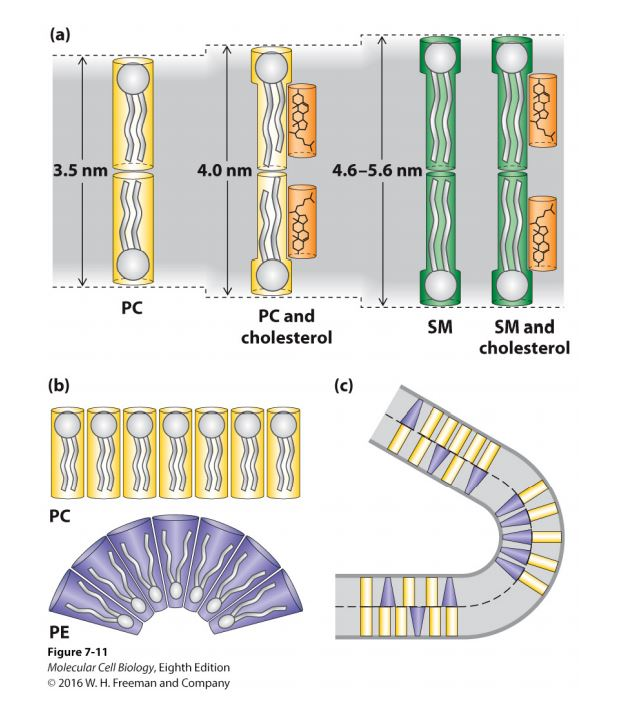
\includegraphics[width=0.5\textwidth]{images/doppiostrato.JPG}
            \caption{\small volume della membrana in relazione a lipidi differenti}
            \label{fig:mesh1}
        \end{figure}
        
        In base alle componenti dei foglietti lipidici, la membrana assume conformazione e spessore differente:
        \begin{itemize}
            \item un doppio strato di fosfatidil colina combinato con degli steroli aumenta lo spessore rispetto a un doppio strato di fosfatidil colina semplice
            \item un doppio strato di sfingomielina combinato con degli steroli \textit{non} aumenta lo spessore rispetto a un doppio strato di sfingomielina semplice. Essendo la sfingomielina \textit{un cilindro più alto}, questo doppio strati risulta più spesso di quello di fosfatidil colina.
            \item la presenza di fosfatidil etanolammina induce un ripiegamento.
        \end{itemize}
        
        Esistono processi che permettono una temporanea formazione di zattere lipidiche (composizione specifica locale di lipidi) per specializzazioni della membrana per veicolare informazioni.
    
\section{Proteine di membrana}
    \small
    Ogni membrana incorpora delle proteine con funzionalità specifiche.
    \subsection{Tipologie di proteine di membrana}
        Le proteine di membrana possono essere integrali, ancorate a lipidi o periferiche di membrana. Molto raramente si può trattare di un $\alpha E$ associata ad un mono-strato.
        
         \begin{figure}[h]
            \centering
            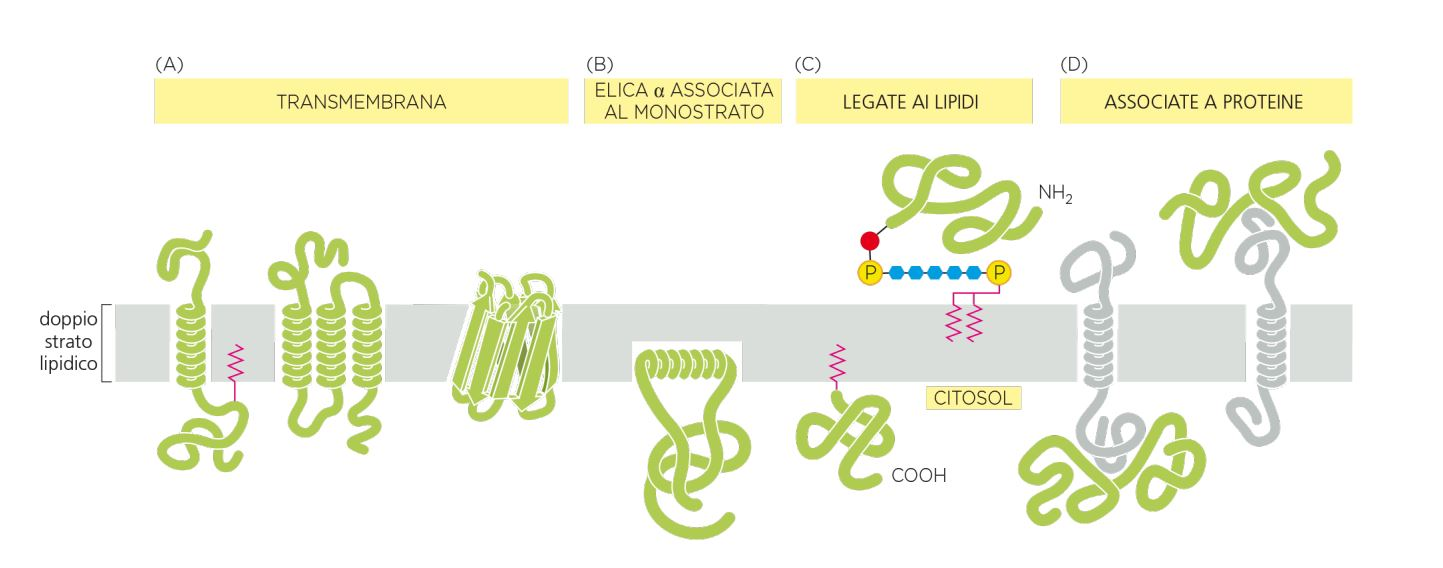
\includegraphics[width=1\textwidth]{images/proteinemembrana.JPG}
            \caption{\small tipologie di proteine di membrana}
            \label{fig:mesh1}
        \end{figure}
        
        \subsubsection{Integrali di membrana}
            Consistono di tre domini:
            \begin{enumerate}
                \item transmembrana: la porzione che effettivamente attraversa il doppio strato lipidico.
                \item luminale o extracellulare: il dominio che volge sul lumen o all'esterno della cellula
                \item citosolico: la parte che si interfaccia con il citosol
            \end{enumerate}
            Attraversano da parte a parte la membrana una (\textit{single pass}) o più volte (\textit{multi pass}). Un passaggio è composto di un'elica di circa 20/25 AA (a seconda della composizione della membrana attraversa spessori differenti).\\
            La conformazione dell'$\alpha$E è tale da lasciare all'esterno dell'elica le catene AA che solitamente sono idrofobiche per rimanere associata alla membrana, i legami H sono invece interni all'elica protetti dall'ambiente idrofobico.\\
            Tipicamente l'$\alpha$E termina con AA polari, verso la faccia citosolica carichi positivamente mentre sulla faccia extracellulare negativamente.
            Le teste polari dei lipidi di membrana seguono la stessa "regola", quindi il foglietto citosolico è carico positivamente e quello esterno negativamente.\\
            Di seguito degli esempi di proteine transmembrana costituite di $\alpha E$:
            \begin{itemize}
                \item {Glicoforina a dimero}:
                La struttura di questa proteina presa singolarmente attraversa la membrana tramite una sola $\alpha$E (single pass), la sua struttura quaternaria è composta da due di queste molecole.
                L'associazione di due proteine è promossa dall'interazione delle due $\alpha$E per formare un coiled-coil a livello trasnmembrana (interazioni van der Waals tra le due eliche).
                \item{Acuaporina}:
                L'acquaporina è un esempio di proteina multi pass: la struttura terziaria è composta di sei $\alpha$E transmembrana diagonali ad essa, quella quaternaria comprende quattro di questi domini e permette la formazione di canali acquosi. All'interno quindi sono presenti residui AA idrofili.
                La proteina completa è formata da quattro di queste molecole.
                \item{Rodopsina}:
                La rodopsina è un esempio di proteina batterica multipass composta di sette $\alpha$E transmembrana perpendicolari ad essa.
                \item{TRC (\textit{T-cell-receptor})}:
                è una struttura che consiste di complessi carichi interni alle $\alpha$E in modo che si associno perchè energicamente favorite.
            \end{itemize}
            Un canale transmembrana costituito di F$\beta$ sono le porine: sono strutturate a \textit{barile} $\beta$, le componenti transmembrana sono idrofiliche verso l'interno e idrofobiche verso l'esterno. 
            Il backbone presenta legami covalenti polari che vengono preservati dall'ambiente idrofobico grazie alle interazioni H interne alla porina. Generalmente le proteine di membrana con F$\beta$ sono più rigide.
            
        \subsubsection{Ancorate a lipidi}
            Le proteine ancorate ai lipidi non possiedono una porzione proteica ancorata al doppio strato, bensì sono solamente affacciati sul citosol o sulla porzione extracellulare.
            Sono tipicamente globulari, sono associate irreversibilmente alla membrana perchè legate ai lipidi tramite una delle seguenti reazioni:
            \begin{itemize}
                \item alcilazione (solitamente su N-terminale con miristato o palmitato)
                \item prenilazione (solitamente su C-terminale con farnesile o geranil-geranile)
                \item GPI anchor (\textit{glicosil fosfatidil inositolo}, un glicolipide, componente saccaridica si lega alla proteina), tipicamente extracellulari e determina l'ancoraggio della proteina (C-terminale) al GPI.
            \end{itemize}
            \textbf{Proteine e lipidi glicosilati}\\
                A livello della membrana sono comprese anche proteine e lipidi glicosilati associati alla membrana che possono conferire proprietà meccanica, sono usati anche per riconoscimento e adesione. \\
                Ad esempio i gruppi sanguigni umani sono oligosaccaridi (cinque monosaccaridi di base) ancorati sul lato extracellulare della membrana. Hanno una configurazione di base alla quale possono aggiungersi precisi monosaccaridi per determinare i gruppi A o B. \\
                Nelle cellule eucariotiche il \textit{cortex} (costituito in larga parte di \textit{spettrina} nel caso del globulo rosso) che forma reticolo sulla faccia citoplasmatica che si associa ad altre proteine transmembrana e ne conferisce determinate proprietà meccaniche (rigidità e forma). Gli elementi associati allo strato lipidico e alle componenti citoschelettrici (come la spettrina) possono avere mobilità limitata.
            
        \subsubsection{Periferiche di membrana}
            Sono associate temporaneamente alla membrana tramite legami non covalenti, per esempio possono associarsi ad altre proteine transmembrana o direttamente alle teste polari dei lipidi. \\
            Ad esempio, le fosfolipasi sono proteine che si associano ai lipidi che idrolizzano legami specifici e dissociare componenti (nel caso in cui non siano più funzionali o non necessarie). 
            Le fosfolipasi possono essere presenti anche in ambiente citosolico senza essere legate alla membrane. Sono usate sperimentalmente su cellule intatte per verificare la composizione del foglio esterno della membrana.
            
    \subsection{Detergenti}
        Al fine di studiare le componenti proteiche facenti parte della membrana cellulare, è possibile utilizzare un mezzo per estrarle tramite solubilizzazione, ovvero un \textit{detergente}.\\ 
        I detergenti sono sostanze anfipatiche che stabilizzano la porzione idrofoba della proteina. Possono essere ionici o non-ionici.
        \subsubsection{Ionici}
            Sono detergenti "aggressivi", talvolta sono "troppo" efficaci al fine dell'estrazione della proteina perchè possono portare alla denaturazione della proteina. Formano una micella attorno alla proteina. Un esempio è \textit{SDS}, che ha carica netta e viene associato ad uno ione.
        \subsubsection{Non-ionici}
            Sono detergenti con una polarità ma non una carica netta, questo permette di evitare la denaturazione della proteine, dissolvendo le proteine ma non formando micelle nette. 
            Sopra una certa concentrazione del detergente anche in questo caso di va incontro alla formazione di una micella: si parla di \textit{CMC}, ovvero \textit{critical mycell concentration}.
        
    \subsection{Studio delle proteine di membrana senza detergente}
        \subsubsection{FRAP}
            FRAP (\textit{fluorecence recovery after photoblieaching}) è una tecnica che si può usare sperimentalmente per verificare la migrazione dei lipidi sulla membrana. \\
            Il processo consiste nel marcare una determinata proteina di membrana con fluorescenza. Applicando un bleaching (\textbf{sbiancare} la fluorescenza) in un dominio di membrana limitato ("spegnendo" la fluorescenza localmente) si osserva nel tempo la ricomparsa della fluorescenza in quella zona.\\
            La ricomparsa della fluorescenza in rapporto al tempo indica la capacità di migrazione dei lipidi attraverso la membrana, ovvero il \textit{coefficente di diffusione}.
        \subsubsection{SPT o SMT}
            SPT o SMT (\textit{single particle/molecule tracking}) è una tecnica per visualizzare il movimento di una singola molecola nel tempo.\\
            Analizzandone il tracciato si può dedurre se una molecola è libera o ha una bassa motilità.
        
\pagebreak